% !TEX program = xelatex
\documentclass{beamer}
\usepackage{ctex, hyperref}
\usepackage{calligra}
\usepackage{amssymb}
\usepackage[T1]{fontenc}
\usepackage{listings}
\usepackage{multicol}
\usepackage{bookmark}

\definecolor{mygreen}{rgb}{0,0.6,0}
\definecolor{mygray}{rgb}{0.5,0.5,0.5}
\definecolor{mymauve}{rgb}{0.58,0,0.82}

\lstset{ %
  backgroundcolor=\color{white},      % choose the background color
  basicstyle=\footnotesize\ttfamily,  % size of fonts used for the code
  columns=fullflexible,
  tabsize=2,
  breaklines=true,               % automatic line breaking only at whitespace
  captionpos=b,                  % sets the caption-position to bottom
  commentstyle=\color{mygreen},  % comment style
  escapeinside={\%*}{*)},        % if you want to add LaTeX within your code
  keywordstyle=\color{blue},     % keyword style
  stringstyle=\color{mymauve}\ttfamily,  % string literal style
  frame=none,
  rulesepcolor=\color{red!20!green!20!blue!20},
  % identifierstyle=\color{red},
  language=c++,
}

\ctexset {
  today=old
}
\author{trswnca @ tjuacm}
\title{Data Structure I.}
\subtitle{Basic Manual Data Structure by Example}
\institute{2021 TJU Summer Camp}
\date{\today}
\usepackage{tju-trswnca}

% \AtBeginSubsection[] {
%   \begin{frame}
%     \begin{multicols}{2}
%     \tableofcontents[currentsection,currentsubsection]
%     \end{multicols}
%   \end{frame}
% }

\begin{document}

\begin{frame}
	\titlepage
	\begin{figure}[htpb]
		\begin{center}
			
\includegraphics[width=0.15\linewidth]{pic/tju.png}
		\end{center}
	\end{figure}
\end{frame}

\begin{frame}{Preface}
  数据结构是在计算机中存储、组织数据的方式。
  
  此处数据结构更加偏指通过一些维护操作,使得数据具有更利于答案计算的性质。

\end{frame}

\begin{frame}
\tableofcontents[subsectionstyle=hide]
\end{frame}

\section{Basics}

\begin{frame}
  鉴于过于简单,不会的自学
  \begin{itemize}
    \item Queue: \url{https://oi-wiki.org/ds/stack/}
    \item Stack: \url{https://oi-wiki.org/ds/queue/}
    \item Linked list \url{https://oi-wiki.org/ds/linked-list/}
  \end{itemize}

  具体的应用可以看《算法导论》
\end{frame}

\section{Disjoint Set}
\subsection{Operations}

\begin{frame}[fragile]{Data Structure}
  $fa[i]$ 表示 $i$ 的父亲

  $1 \sim n$ 构成一个森林,每颗树代表一个集合
    
  \begin{block}{Initialization}
  \begin{lstlisting}
const int N = 1e5 + 10;
int fa[N];
void init() { fa[i] = i; }
  \end{lstlisting}
  \end{block}
  
\end{frame}

\begin{frame}[fragile]{Basic Operations}
  \begin{block}{Find}
    \begin{lstlisting}
int find(int x) {
  return x == fa[x] ? x : find(fa[x]);
}
    \end{lstlisting}
  \end{block}

  \begin{block}{Union}
    \begin{lstlisting}
void union(int x, int y) {
  x = find(x), y = find(y);
  fa[x] = y;
}
    \end{lstlisting}
  \end{block}
\end{frame}

\subsection{Extend Operations}

\begin{frame}{Tech}

  并查集可以维护具有\textbf{传递性}的数据

  如果按照不做优化,单次查找会遍历整条树链,复杂度 $O(n)$
  ~\\

  一般有两种优化:

  \begin{itemize}
    \item 路径压缩
    \item 按秩合并
  \end{itemize}

  更多优化:
  
  \url{https://www.zhihu.com/question/28410263/answer/40966441}

\end{frame}

\begin{frame}[fragile]{Compression}
   \begin{columns}[T,onlytextwidth]
    \column{0.37\textwidth}
    \begin{block}{find}
    \begin{lstlisting}
int find(int x) {
  return x == fa[x] ? 
    x : fa[x] = find(x);
}
    \end{lstlisting}
  \end{block}

    \column{0.6\textwidth}
   \begin{figure}
       %\begin{center}
         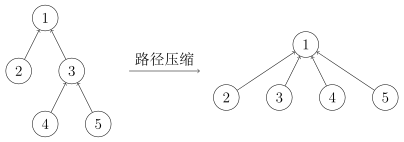
\includegraphics[width=\linewidth]{pic/disjoint-set-compress.png}
       %\end{center}
   \end{figure}
    
  \end{columns}

  ~\\

  这样复杂度为 $O(\alpha (m, n) n)$ 其中 $\alpha (m, n)$ 为反阿克曼函数,一般可以认为小于 $5$
\end{frame}

\begin{frame}[fragile]{Linking by rank}
  我们将一棵点数与深度都较小的集合树连接到一棵更大的集合树下
  \begin{block}{union}
    \begin{lstlisting}
void union(int x, int y) {
  x = find(x), y = find(y);
  if (x == y) return;
  if (size[x] > size[y]) swap(x, y);
  fa[x] = y; size[y] += size[x];
}
    \end{lstlisting}
  \end{block}
\end{frame}

\subsection{Problems}
\begin{frame}[fragile]{BZOJ 3376}
  \begin{block}{Cube Stacking}
    约翰和贝茜在玩一个方块游戏。编号为 $1$ 到 $n$ 的 $n$ 个方块正放在地上.每个构成一个立方柱。
游戏开始后,约翰会给贝茜发出 $m$ 个指令。指令有两种:
\begin{itemize}
  \item 移动:将包含 $x$ 的立方柱移动到包含 $y$ 的立方柱上;
  \item 统计:统计名含 $x$ 的立方柱中,在 $x$ 下方的方块数目。
\end{itemize}
  \end{block}
  
\end{frame}

\begin{frame}[fragile]{BZOJ 3376}
    \begin{block}{Sol.}
    带权并查集,以每堆方块最下面的方块为并查集的树根,记录每堆方块最上面的方块编号,每次合并将 $x$ 块的根的父节点置为 $y$ 所在堆最上面的方块。
    
    记 $d(x)$ 为从 $x$(包含)到 $x$ 的父节点(不包含)之间的方块数量。每次查询将 $d(x)$ 取一个前缀和即可。
  \end{block}

  \textbf{Implement:} \url{https://vjudge.net/solution/31828472}
\end{frame}

\begin{frame}{UVA 11987}
  \begin{block}{Almost Union-Find}
  $n$ 个数,从 $1$ 到 $n$,初始状态分属不同集合

  \begin{itemize}
    \item 合并数字 $p$ 和数字 $q$ 所在的集合
    \item 把 $p$ 插入 $q$ 所在的集合(并在 $p$ 原来所在的集合中删除 $p$)
    \item 询问某个数字 $p$ 所在集合的元素个数以及总和
  \end{itemize}
  \end{block}

\end{frame}

\begin{frame}{UVA 11987}
 \begin{block}{Sol .}
   做一次 \textbf{镜像}
   $f[i] = i + n, f[i + n] = i + n$
 \end{block}
\end{frame}

%\section{ST table}

\section{Leftist\ Tree}
\subsection{Descriptions}
\begin{frame}{Introduction}
  左偏树是一种 \textbf{可并堆},具有堆的性质,并且是「左偏」的,因此可以快速合并。
  
  \pause
  对于一棵二叉树,我们定义 \textbf{外节点} 为左儿子或右儿子为空的节点,定义一个外节点的 $dist$ 为 $1$,一个不是外节点的节点 $dist$ 为其到子树中最近的外节点的距离加一。\textbf{空节点的 $dist$ 为 $0$} 。
  
  「左偏」:每个节点左儿子的 $dist$ 都大于等于右儿子的 $dist$ 。
\end{frame}

\begin{frame}[fragile]{Data Structure}
   \begin{block}{Data}
        \begin{lstlisting}
struct Node {
  int ls, rs, val, d;
}
        \end{lstlisting}
   \end{block}
\end{frame}

\subsection{Operations}
\begin{frame}[fragile]{Merge}
   \begin{block}{Merge}
        \begin{lstlisting}
int merge(int x, int y) { 
  if (!x || !y) return x | y;
  if (t[x].val > t[y].val) swap(x, y); 
  t[x].rs = merge(t[x].rs, y); 
  if (t[t[x].rs].d > t[t[x].ls].d)
    swap(t[x].ls, t[x].rs); 
  t[x].d = t[t[x].rs].d + 1; 
  return x;
}
        \end{lstlisting}
   \end{block}
\end{frame}

\begin{frame}{Merge}

由于左偏性质,每递归一层,其中一个堆根节点的 $\mathrm{dist}$ 就会减小 $1$,而“一棵有 $n$ 个节点的二叉树,根的 $\mathrm{dist}$ 不超过 $\left\lceil\log (n+1)\right\rceil$”,所以合并两个大小分别为 $n$ 和 $m$ 的堆复杂度是 $O(\log n+\log m)$。

\begin{block}{Extended}
\begin{itemize}
    \item 删除根节点 \pause 合并根的左右儿子
    \item 插入节点 \pause 相当于合并只有一个节点的堆
\end{itemize}
\end{block}
    
\end{frame}

\begin{frame}[fragile]{Modify}
   可以维护不改变相对大小的对整个堆的修改,在根打上标记,删除根/合并堆(访问儿子)时下传标记即可
   
   \begin{block}{Modify}
        \begin{lstlisting}
int merge(int x, int y) {
  if (!x || !y) return x | y;
  if (t[x].val > t[y].val) swap(x, y);
  pushdown(x);
  t[x].rs = merge(t[x].rs, y);
  if (t[t[x].rs].d > t[t[x].ls].d) swap(t[x].ls, t[x].rs);
  t[x].d = t[t[x].rs].d + 1;
  return x;
}
int pop(int x) {
  pushdown(x); return merge(t[x].ls, t[x].rs);
}
        \end{lstlisting}
   \end{block}
\end{frame}

\subsection{Problems}

\begin{frame}{Luogu P1456}
    \begin{block}{Monkey King}
        曾经在一个森林中居住着 $N$ 只好斗的猴子。在最初他们互不认识。争吵发生时,双方会邀请它们各自最强壮的朋友并发起决斗。在决斗之后两只猴子和他们各自的伙伴都成为朋友.
        假设每只猴子有一个强壮值,强壮值将在一场决斗后减少为原先的一半.
        给出$M$次争斗,询问每次争斗后最强壮的值。
    \end{block}
    \pause
    \begin{block}{Sol .}
        可合并的大根堆,删除根节点,插入根节点的一半
        
        \textbf{Implement:} \url{https://www.luogu.com.cn/record/54354821}
    \end{block}
\end{frame}



\section{Trie\ Tree}

\subsection{Descriptions}

\begin{frame}[fragile]
Trie树是用链代表字符串,节点维护信息的树

\begin{figure}
  \centering
  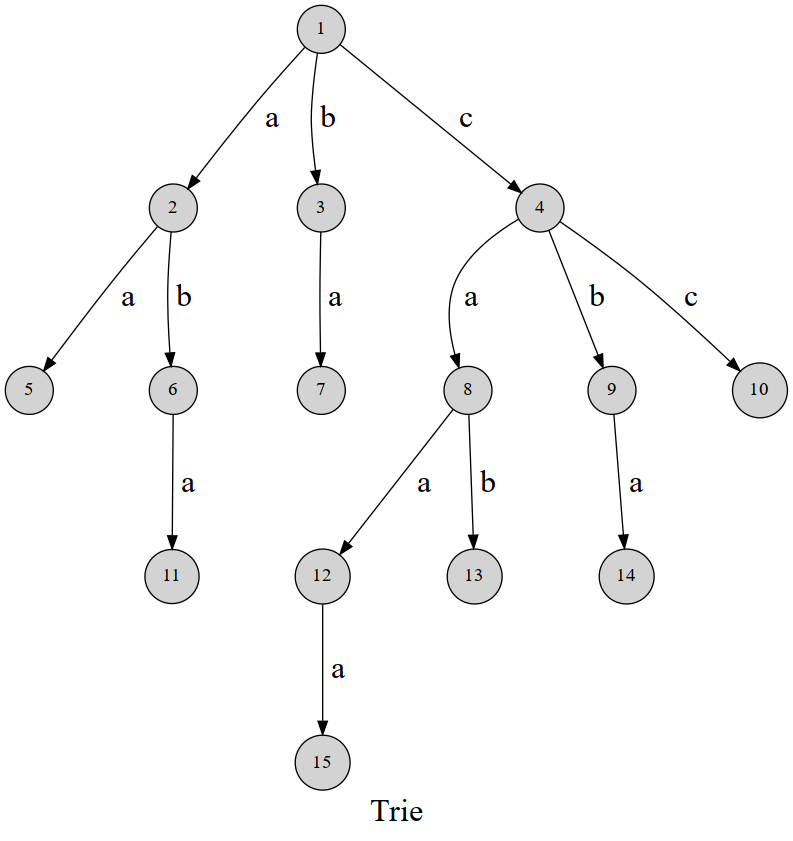
\includegraphics[scale=0.20]{pic/trie1.png}
\end{figure}

\end{frame}



\begin{frame}[fragile]{Data Structure}
  \begin{block}{Data}
    \begin{lstlisting}
const int N = 1e5 + 10;
const int M = 26;
int ch[N * M][M], tot;
    \end{lstlisting}
  \end{block}
  $ch[x][i]$ 存 $x$ 节点的按字典序第 $i$ 个儿子
  
  如果子节点为空,则 $ch[x][i] = 0$
\end{frame}

\begin{frame}[fragile]{Operations}
  \begin{block}{Insert}
    \begin{lstlisting}
void insert(char s[]) {
  int n = strlen(s), x = 0;
  for (int i = 0; i < n; ++ i) {
    if (!ch[x][s[i] - 'a']) ch[x][s[i] - 'a'] = ++tot;
    x = ch[x][s[i] - 'a']; val[x] ++;
  }
}
    \end{lstlisting}
  \end{block}

  $val$ 可以维护子树内信息,具有前缀和性质的信息

  \begin{itemize}
    \item 前缀个数
    \item 子树最小值
    \item $\cdots$
  \end{itemize}
\end{frame}

\begin{frame}[fragile]{Operations}
  \begin{block}{Query}
    \begin{lstlisting}
bool query(char s[]) {
  int n = strlen(s), x = 0;
  for (int i = 0; i < n; ++ i) {
    if (!ch[x][s[i] - 'a']) return false;
    x = ch[x][s[i] - 'a'];
  }
  return true;
}
    \end{lstlisting}
  \end{block}

  询问的值可以根据 $val$ 的设置调整
\end{frame}

\subsection{Problems}

\begin{frame}{Luogo P4551}
  \begin{block}{最长异或路径}
    给定一棵 $n$ 个点的带权树,结点下标从 $1$ 开始到 $N$。寻找树中找两个结点,求最长的异或路径。

异或路径指的是指两个结点之间唯一路径上的所有边权的异或。

  \end{block}

  \pause
  \begin{block}{Sol.}
    通过异或前缀和求一段连续区间异或

    到根节点只有 $n$ 个前缀,全部插入,再走一遍进行查询即可

  \textbf{Implement:} \url{https://www.luogu.com.cn/record/53774710}
  \end{block}
\end{frame}

\section{Fenwick\ Tree}

\subsection{Descriptions}

\begin{frame}{Introduction}
树状数组就是用数组来模拟树形结构,因为写法简洁,所以很多能使用树状数组解决的问题不用建树解决.

树状数组可以解决大部分基于区间上的更新以及求和问题,修改和查询的复杂度都是$O(logN)$.
\end{frame}


\begin{frame}[fragile]{Data Structure}
  \begin{block}{Data}
    \begin{lstlisting}
const int N = 1e5 + 10;
int C[N];
    \end{lstlisting}
  \end{block}
  $C[x]$ 储存 $$\displaystyle \sum_{k = x - \operatorname{lowbit}(x)}^x a[k]$$ 
  
  $\operatorname{lowbit}(x) = x \& -x$ 表示二进制表示下,最低位为 $1$ 的数
\end{frame}

\subsection{Operations}


\begin{frame}[fragile]{Query}
  \begin{block}{Query}
  这里说的查询是查询任一区间的和,由于区间和具有可加减性,故转化为求前缀和;

查询前缀和就是把大区间分成几段长度不等的小区间,然后求和。区间的个数为$O(logn)$,所以查询的时间复杂度为$O(logn)$。
    \begin{lstlisting}
int query(int *C, int n, int x) {
  int res = 0;
  for (; x > 0; x -= x & -x) res += C[x];
  return res;
}
    \end{lstlisting}
  \end{block}
\end{frame}

\begin{frame}[fragile]{Add}
  \begin{block}{Add}
  更新的时候只要更新修改某个点会影响到哪些数组
    \begin{lstlisting}
void update(int *C, int n, int x, int val) {
  for (; x <= n; x += x & -x) C[x] += val;
}
    \end{lstlisting}
  \end{block}
\end{frame}

\subsection{Problems}
\begin{frame}[shrink]{LOJ 130, 131, 132}
  \begin{block}{树状数组模板3题}
      \begin{itemize}
          \item 130:单点修改,单点询问
          \item 131:区间修改,单点查询
          \item 132:区间修改,区间查询
      \end{itemize}
  \end{block}

  \pause
  \begin{block}{Sol.}
  \begin{itemize}
      \item 130:\textbf{Implement:} \url{https://loj.ac/s/858312}
      \item 131:差分后求和即可 \\
        \textbf{Implement:} \url{https://loj.ac/s/858367}
      \item 132:维护两个差分数组 \\
         \textbf{Implement:} \url{https://loj.ac/s/858505}
  \end{itemize}
  \end{block}

\end{frame}



\section{Segment Tree}

\subsection{Descriptions}

\begin{frame}[fragile]{Data Structure}
线段树维护一个区间(且能区间合并)的信息,所以一般需要维护 \textbf{是哪个区间} \textbf{区间信息}

\href{run:线段树基础.pdf}{线段树基础}

如果空间要求比较严苛,可以省略区间 $[l, r]$ 的记录,递归时带区间范围

\begin{block}{Data}
  \begin{lstlisting}
const int N = 1e5 + 10;
struct Node {
  int l, r, val, tag;
} t[N << 2];
  \end{lstlisting} 
\end{block}

\end{frame}

\subsection{Problems}
\begin{frame}{Problem A}
  \begin{problem}
维护一个长度为 $n$ 的序列:

\begin{itemize}
    \item 区间 $[l, r]$ 加上 $x$
    \item 区间 $[l, r]$ 乘上 $x$
    \item 查询区间和
\end{itemize}
  ~\\
  \pause 先加再乘还是先乘再加?
  \end{problem}
\end{frame}

\begin{frame}{先加再乘}
    $(val, add, mul) \odot (ad, mu)$
    $(val + add) \times mul \longrightarrow [(val + add) \times mul + ad] \times mu$
    \pause
    那么 $$\begin{cases} add' &= add + ad / mu \\ mul' &= mul \times mu \end{cases}$$
\end{frame}

\begin{frame}{先乘再加}
    $(val, add, mul) \odot (ad, mu)$
    $val\times mul + add \times (r -l + 1) \longrightarrow (val \times mul + add \times (r -l + 1)) \times mu + ad$
    \pause
    那么 $$\begin{cases} add' &= add \times mu + ad \\ mul' &= mul \times mu\end{cases}$$
\end{frame}

\begin{frame}{Problem B}
维护一个长度为 $n$ 的序列:

\begin{itemize}
    \item 区间 $[l, r]$ 加上 $a_i$
    \item 区间 $[l, r]$ 加上 $1$
    \item 区间 $[l, r]$ 置为 $x$
    \item 查询区间和
\end{itemize}
\end{frame}

\begin{frame}{Sol .}
    $val$ 当前节点表示的区间和
    
    $add1$ 第一种操作值
    
    $add2$ 第二种操作值
    
    $flag$ 是否覆盖,不覆盖为 $-1$
\end{frame}

\begin{frame}{Luogu P3605}
\begin{block}{Promotion Counting P}
给出一颗带权树,询问有多少数对,满足孩子的值大于祖先.
\end{block}

\pause
\begin{block}{Sol .}
如果一颗维护了子树的权值信息,那么对于权值为 $x$ 的点,只需要查询 $x+1 \sim n$ 的数量即可.

如果自底向上递归,不断合并线段树维护子树权值,即可求出所有数量.

具体来说, 只需要选择一个节点,把另外一个节点的值加过来,即可完成

\textbf{Implement:} \url{http://blog.trswnca.top/index.php/archives/72/}
\end{block}
\end{frame}


\begin{frame}{Extended}
   事实上,只要是能够区间合并的信息都可以用线段树维护
   ~\\
   如:和、积、最值、矩阵乘积、gcd、线性基、bitset、hash
\end{frame}

\begin{frame}
\begin{center}
{\Huge\calligra Thanks!}
\end{center}
\end{frame}

\end{document}